\documentclass[onecolumn, compsoc,11pt]{IEEEtran}
\let\labelindent\relax
\usepackage{enumitem}
\usepackage{etex}
\usepackage{amssymb,amsfonts,amsmath,amsthm}
\usepackage{graphicx}
 \usepackage[usenames,x11names, dvipsnames, svgnames]{xcolor}
\usepackage{amsmath,amssymb}
\usepackage{dsfont}
\usepackage{mathrsfs}
\usepackage{hyperref}
\hypersetup{
    colorlinks=true,
    linkcolor=black,
    citecolor=MediumBlue,
    filecolor=black,
    urlcolor=DodgerBlue4,
    breaklinks=false,
%linkbordercolor=red,% hyperlink borders will be red
  %pdfborderstyle={/S/U/W 1}% border style will be underline of width 1pt
}
\usepackage{array}
%\usepackage{multirow}    
%\usepackage[T1,euler-digits]{eulervm}
%\usepackage{times}
%\usepackage{pxfonts}
\usepackage{tikz}
\usepackage{pgfplots}
\usetikzlibrary{shapes,calc,shadows,fadings,arrows,decorations.pathreplacing,automata,positioning}
\usetikzlibrary{external}
\usetikzlibrary{decorations.text}
\tikzexternalize[prefix=./Figures/External/]% activate externalization!
\tikzexternaldisable
%\addtolength{\voffset}{.1in}  
\usepackage{geometry}
\geometry{a4paper, left=.65in,right=.65in,top=.8in,bottom=0.8in}

\addtolength{\textwidth}{-.1in}    
\addtolength{\hoffset}{.05in}    
\addtolength{\textheight}{.1in}    
\addtolength{\footskip}{0in}    
\usepackage{rotating}
 \definecolor{nodecol}{RGB}{240,240,220}
 \definecolor{nodeedge}{RGB}{240,240,225}
  \definecolor{edgecol}{RGB}{130,130,130}
    \tikzset{%
fshadow/.style={      preaction={
         fill=black,opacity=.3,
         path fading=circle with fuzzy edge 20 percent,
         transform canvas={xshift=1mm,yshift=-1mm}
       }} 
}
\usetikzlibrary{pgfplots.dateplot}
 \usetikzlibrary{patterns}
\usetikzlibrary{decorations.markings}
\usepackage{fancyhdr}
\usepackage{mathtools}
\usepackage{datetime}
\usepackage{comment}
%% ## Equation Space Control---------------------------
\def\EQSP{2pt}
\newcommand{\mltlne}[2][\EQSP]{\begingroup\setlength\abovedisplayskip{#1}\setlength\belowdisplayskip{#1}\begin{equation}\begin{multlined} #2 \end{multlined}\end{equation}\endgroup}
\newcommand{\cgather}[2][\EQSP]{\begingroup\setlength\abovedisplayskip{#1}\setlength\belowdisplayskip{#1}\begin{gather} #2 \end{gather}\endgroup}
\newcommand{\cgathers}[2][\EQSP]{\begingroup\setlength\abovedisplayskip{#1}\setlength\belowdisplayskip{#1}\begin{gather*} #2 \end{gather*}\endgroup}
\newcommand{\calign}[2][\EQSP]{\begingroup\setlength\abovedisplayskip{#1}\setlength\belowdisplayskip{#1}\begin{align} #2 \end{align}\endgroup}
\newcommand{\caligns}[2][\EQSP]{\begingroup\setlength\abovedisplayskip{#1}\setlength\belowdisplayskip{#1}\begin{align*} #2 \end{align*}\endgroup}
\newcommand{\mnp}[2]{\begin{minipage}{#1}#2\end{minipage}} 
%% COLOR DEFS------------------------------------------
\newtheorem{thm}{Theorem}
\newtheorem{cor}{Corollary}
\newtheorem{lem}{Lemma}
\newtheorem{prop}{Proposition}
\newtheorem{defn}{Definition}
\newtheorem{example}{Example}
\newtheorem{rem}{Remark}
\newtheorem{notn}{Notation}
%%------------PROOF INCLUSION -----------------
\def\NOPROOF{Proof omitted.}
\newif\ifproof
\prooffalse % or \draftfalse
\newcommand{\Proof}[1]{
\ifproof
\begin{IEEEproof}
#1\end{IEEEproof}
\else
\NOPROOF
\fi
 }
%%------------ -----------------
\newcommand{\DETAILS}[1]{#1}
%%------------ -----------------
% color commands------------------------
\newcommand{\etal}{\textit{et} \mspace{3mu} \textit{al.}}
% \renewcommand{\algorithmiccomment}[1]{$/** $ #1 $ **/$}
\newcommand{\vect}[1]{\textbf{\textit{#1}}}
\newcommand{\figfont}{\fontsize{8}{8}\selectfont\strut}
\newcommand{\hlt}{ \bf \sffamily \itshape\color[rgb]{.1,.2,.45}}
\newcommand{\pitilde}{\widetilde{\pi}}
\newcommand{\Pitilde}{\widetilde{\Pi}}
\newcommand{\bvec}{\vartheta}
\newcommand{\algo}{\textrm{\bf\texttt{GenESeSS}}\xspace}
\newcommand{\xalgo}{\textrm{\bf\texttt{xGenESeSS}}\xspace}
\newcommand{\FNTST}{\bf }
\newcommand{\FNTED}{\color{darkgray} \scriptsize $\phantom{.}$}
\renewcommand{\baselinestretch}{.95}
\newcommand{\sync}{\otimes}
\newcommand{\psync}{\hspace{3pt}\overrightarrow{\hspace{-3pt}\sync}}
%\newcommand{\psync}{\raisebox{-4pt}{\begin{tikzpicture}\node[anchor=south] (A) {$\sync$};
%\draw [->,>=stealth] ([yshift=-2pt, xshift=2pt]A.north west) -- ([yshift=-2pt]A.north east); %\end{tikzpicture}}}
\newcommand{\base}[1]{\llbracket #1 \rrbracket}
\newcommand{\nst}{\textrm{\sffamily\textsc{Numstates}}}
\newcommand{\HA}{\boldsymbol{\mathds{H}}}
\newcommand{\eqp}{ \vartheta }
\newcommand{\entropy}[1]{\boldsymbol{h}\left ( #1 \right )}
\newcommand{\norm}[1]{\left\lVert #1 \right\rVert}%
\newcommand{\abs}[1]{\left\lvert #1 \right\rvert}%
\newcommand{\absB}[1]{\big\lvert #1 \big\rvert}%
% #############################################################
% #############################################################
% PREAMBLE ####################################################
% #############################################################
% #############################################################
% \usepackage{pnastwoF}
\DeclareMathOperator*{\argmax}{argmax}
\newcommand{\ND}{ \mathcal{N}  }
\usepackage[linesnumbered,ruled,vlined,noend]{algorithm2e}
\newcommand{\captionN}[1]{\caption{\color{darkgray} \sffamily \fontsize{8}{10}\selectfont #1  }}
\newcommand{\btl}{\ \textbf{\small\sffamily bits/letter}}
\usepackage{txfonts}
%\usepackage{ccfonts}
%%% save defaults
\renewcommand{\rmdefault}{phv} % Arial
\renewcommand{\sfdefault}{phv} % Arial
\edef\keptrmdefault{\rmdefault}
\edef\keptsfdefault{\sfdefault}
\edef\keptttdefault{\ttdefault}

%\usepackage{kerkis}
\usepackage[OT1]{fontenc}
\usepackage{concmath}
%\usepackage[T1]{eulervm}
%\usepackage[OT1]{fontenc}
%%% restore defaults
\edef\rmdefault{\keptrmdefault}
\edef\sfdefault{\keptsfdefault}
\edef\ttdefault{\keptttdefault}
\tikzexternalenable
% ##########################################################
\tikzfading[name=fade out,
            inner color=transparent!0,
            outer color=transparent!100]
%###################################
\newcommand{\xtitaut}[2]{
\noindent\mnp{\textwidth}{
\mnp{\textwidth}{\raggedright\Huge \bf \sffamily #1}

\vskip 1em

{\bf \sffamily #2}
}
\vskip 2em
}
%###################################
%###################################
\tikzset{wiggle/.style={decorate, decoration={random steps, amplitude=10pt}}}
\usetikzlibrary{decorations.pathmorphing}
\pgfdeclaredecoration{Snake}{initial}
{
  \state{initial}[switch if less than=+.625\pgfdecorationsegmentlength to final,
                  width=+.3125\pgfdecorationsegmentlength,
                  next state=down]{
    \pgfpathmoveto{\pgfqpoint{0pt}{\pgfdecorationsegmentamplitude}}
  }
  \state{down}[switch if less than=+.8125\pgfdecorationsegmentlength to end down,
               width=+.5\pgfdecorationsegmentlength,
               next state=up]{
    \pgfpathcosine{\pgfqpoint{.25\pgfdecorationsegmentlength}{-1\pgfdecorationsegmentamplitude}}
    \pgfpathsine{\pgfqpoint{.25\pgfdecorationsegmentlength}{-1\pgfdecorationsegmentamplitude}}
  }
  \state{up}[switch if less than=+.8125\pgfdecorationsegmentlength to end up,
             width=+.5\pgfdecorationsegmentlength,
             next state=down]{
    \pgfpathcosine{\pgfqpoint{.25\pgfdecorationsegmentlength}{\pgfdecorationsegmentamplitude}}
    \pgfpathsine{\pgfqpoint{.25\pgfdecorationsegmentlength}{\pgfdecorationsegmentamplitude}}
  }
  \state{end down}[width=+.3125\pgfdecorationsegmentlength,
                   next state=final]{
     \pgfpathcosine{\pgfqpoint{.15625\pgfdecorationsegmentlength}{-.5\pgfdecorationsegmentamplitude}}
     \pgfpathsine{\pgfqpoint{.15625\pgfdecorationsegmentlength}{-.5\pgfdecorationsegmentamplitude}}
  }
  \state{end up}[width=+.3125\pgfdecorationsegmentlength,
                 next state=final]{
     \pgfpathcosine{\pgfqpoint{.15625\pgfdecorationsegmentlength}{.5\pgfdecorationsegmentamplitude}}
     \pgfpathsine{\pgfqpoint{.15625\pgfdecorationsegmentlength}{.5\pgfdecorationsegmentamplitude}}
  }
  \state{final}{\pgfpathlineto{\pgfpointdecoratedpathlast}}
}
%###################################
%###################################
\newcolumntype{L}[1]{>{\rule{0pt}{2ex}\raggedright\let\newline\\\arraybackslash\hspace{0pt}}m{#1}}
\newcolumntype{C}[1]{>{\rule{0pt}{2ex}\centering\let\newline\\\arraybackslash\hspace{0pt}}m{#1}}
\newcolumntype{R}[1]{>{\rule{0pt}{2ex}\raggedleft\let\newline\\\arraybackslash\hspace{0pt}}m{#1}}




\newcommand{\drhh}[8]{
\begin{axis}[semithick,
font=\bf \sffamily \fontsize{7}{7}\selectfont,
name=H2,
at=(#4), anchor=#5,
xshift=.3in,
yshift=-.3in,
width=\WDT, 
height=\HGT, 
title={{\LARGE G } ROC area distribution (Out-of-sample)}, 
title style={align=right, },legend cell align=left,
legend style={ xshift=3.5in, yshift=-.6in, draw=white, fill= gray, fill opacity=0.2, 
text opacity=1,},
axis line style={black!80, opacity=0,   thick,,ultra thin, rounded corners=0pt},
axis on top=false, 
xlabel={ROC area},
ylabel={probability},
ylabel style={yshift=-.25in},
xlabel style={yshift=.1in},
grid style={dashed, gray!50},
%grid,
axis background/.style={top color=gray!1,bottom color=gray!2},
enlargelimits=false, 
scale only axis=true,
ymin=0,
%xmin=.7,xmax=1.0,
ylabel style={yshift=.05in},
major tick length=0pt,yticklabel style={/pgf/number format/fixed,/pgf/number format/precision=2},xticklabel style={/pgf/number format/fixed,/pgf/number format/precision=2},
#7,
 ]
\addplot [
    fill=#8,
    thick,
    draw=white,
    opacity=1,
    hist={density,bins=10},
] table [y index=#3] {#1};
% \addlegendentry{$\Delta$ ROC};
\addplot [very thick, Red2,, opacity=.95] gnuplot [raw gnuplot] {plot '#1' u #2:(1./#6.) smooth kdensity};
%
%\draw[thin,black ] (axis cs:.89291,\pgfkeysvalueof{/pgfplots/ymin}) -- (axis cs:.89291,\pgfkeysvalueof{/pgfplots/ymax}) node [midway,right, pos=0.2] {89.3\%};
% \addlegendentry{kde};
\end{axis}
}


\newcommand{\erhh}[6]{
  \begin{axis}[semithick,
font=\bf \sffamily \fontsize{7}{7}\selectfont,
name=H2,
at=(#3), anchor=#4,
xshift=.3in,
yshift=-.3in,
width=\WDT, 
height=\HGT, 
title style={align=center, },legend cell align=left,
legend style={ xshift=3.5in, yshift=-.6in, draw=white, fill= gray, fill opacity=0.2, 
text opacity=1,},
axis line style={black!80, opacity=0,   thick,,ultra thin, rounded corners=0pt},
axis on top=false, 
xlabel={ROC area},
ylabel={probability},
ylabel style={yshift=-.25in},
xlabel style={yshift=.1in},
grid style={dashed, gray!50},
%grid,
axis background/.style={top color=gray!1,bottom color=gray!2},
enlargelimits=false, 
scale only axis=true,
%ymin=0, 
%xmin=.7,xmax=1.0,
ylabel style={yshift=.05in},
major tick length=0pt,yticklabel style={/pgf/number format/fixed,/pgf/number format/precision=2},xticklabel style={/pgf/number format/fixed,/pgf/number format/precision=2},
#5,
 ]
    \addplot[semithick, #6]
    table[x expr=(\coordindex+1),y expr=(\thisrowno{#2})] {#1};
    % \addlegendentry{Cullman, Alabama};
  \end{axis}
}
%################################################
%################################################
%################################################
%################################################
\def\DISCLOSURE#1{\def\disclosure{#1}}
\DISCLOSURE{\raisebox{15pt}{$\phantom{XxxX}$This sheet contains proprietary information 
 not to be released to third parties except for the explicit purpose of evaluation.}
}
 
\usetikzlibrary{arrows}
\usepackage{geometry}
\geometry{a4paper, left=.7in,right=.75in,top=.8in,bottom=0.65in}
\usepackage{textcomp}
\usepackage{colortbl}
% \usepackage{subfigure}
\usepackage{array}
\usepackage{courier}
\usepackage{wrapfig}
\usepackage{pifont}
\usepackage{subfig}
\usetikzlibrary{chains,backgrounds}
\usetikzlibrary{intersections}
\usepackage[super]{cite}  
\usepackage{setspace} 
\makeatletter \renewcommand{\@citess}[1]{\raisebox{1pt}{\textsuperscript{[#1]}}} \makeatother
\usepackage{xstring}
\usepackage{xspace}
\usepgfplotslibrary{groupplots}

\captionsetup[subfigure]{labelformat=empty}
\makeatletter
\renewcommand\section{\@startsection {section}{1}{\z@}%
  {-1ex \@plus -1ex \@minus -.2ex}%
  {0.05ex \@plus.1ex}%
  {\large\bfseries\scshape}}
\renewcommand\subsection{\@startsection {section}{1}{\z@}%
  {-1ex \@plus -.25ex \@minus -.2ex}%
  {0.1ex \@plus.0ex}%
  {\fontsize{11}{10}\selectfont\bfseries\sffamily\color{DodgerBlue4}}}
\renewcommand\subsubsection{\@startsection {section}{1}{\z@}%
  {0ex \@plus -.5ex \@minus -.2ex}%
  {0.0ex \@plus.5ex}%
  {\fontsize{10}{10}\selectfont\bfseries\sffamily\color{Red4}}}
\renewcommand\paragraph{\@startsection {section}{1}{\z@}%
  {-1.5ex \@plus -.5ex \@minus -.2ex}%
  {0.0ex \@plus.5ex}%
  {\fontsize{11}{11}\selectfont\itshape\sffamily\color{Red1!50!black}}}
 

\makeatother
\makeatletter
\pgfdeclareradialshading[tikz@ball]{ball}{\pgfqpoint{-10bp}{10bp}}{%
  color(0bp)=(tikz@ball!30!white);
  color(9bp)=(tikz@ball!75!white);
  color(18bp)=(tikz@ball!90!black);
  color(25bp)=(tikz@ball!70!black);
  color(50bp)=(black)}
\makeatother
\newcommand{\tball}[1][CadetBlue4]{${\color{#1}\Large\boldsymbol{\blacksquare}}$}
\renewcommand{\baselinestretch}{1.05}
\renewcommand{\captionN}[1]{\caption{\color{CadetBlue4!80!black} \sffamily \fontsize{10}{11}\selectfont #1  }}
\tikzexternaldisable 
\parskip=7pt
\parindent=0pt
\newcommand{\Mark}[1]{\textsuperscript{#1}}
% \lhead{\sf\footnotesize \color{DodgerBlue4!70!black}\today}
\pagestyle{fancy} 
\def\COLA{black}
% ###################################
\cfoot{\bf\sffamily \scriptsize \color{Maroon!50} \disclosure }
% \cfoot{}
\lhead{}
\rhead{\scriptsize\bf\sffamily\thepage}
\newcommand{\partxt}{\bf\sffamily\itshape}
% ############################################################
\newif\iftikzX
\tikzXtrue 
% \tikzXfalse
\tikzexternalenable
\def\jobnameX{yfa}
\newcommand{\SPX}[1][50pt]{\vspace{#1}}
% ############################################################
\newcommand{\incomplete}{\colorbox{Red1!80}{\textbf{\footnotesize\color{white}(incomplete section)}}}
\def\FWN{\textbf{\small FWN}\xspace}
% ############################################################
% ##################################
% ##################################
\begin{document} 
% 
\lhead{DARPA Seedling}
\setcounter{page}{4}

\tableofcontents
\clearpage

% \setcounter{page}{1}


\tikzexternaldisable

\begin{tikzpicture}
  \node[] (A) at (0,0) {};
  \foreach\x in {2008,2009,...,2012}{%
    \pgfmathtruncatemacro\y{\x + 4}
    \def\name{TERROR\x}
    \def\nameB{_\y}
    \def\nameC{mean_gammascatter}
    \def\nameD{mean_gammascatter2}
    \node[anchor=north,label={[yshift=-.2in]90:\y}] (A) at (A.south) {\includegraphics[height=1.5in]{../TERRORcomp2/plots/\name\nameB\nameC}};
    \node[anchor=west,label={[yshift=-.2in]90:\y}] (B) at (A.east) {\includegraphics[height=1.5in]{../TERRORcomp2/plots/\name\nameB\nameD}};
  }% 
\end{tikzpicture}



\begin{tikzpicture}
  \node[] (A) at (0,0) {};
  \foreach\x in {2008,2009,...,2012}{%
    \pgfmathtruncatemacro\y{\x + 4}
    \def\name{TERROR\x}
    \def\nameB{_\y}
    \def\nameC{mean_gammahex}
    \def\nameD{mean_gammahex2}
    \node[anchor=north,label={[yshift=-.2in]90:\y}] (A) at (A.south) {\includegraphics[height=1.5in]{../TERRORcomp2/plots/\name\nameB\nameC}};
    \node[anchor=west,label={[yshift=-.2in]90:\y}] (B) at (A.east) {\includegraphics[height=1.5in]{../TERRORcomp2/plots/\name\nameB\nameD}};
  }% 
\end{tikzpicture}


\clearpage

\begin{tikzpicture}
  \node[] (A) at (0,0) {};
    \def\name{CRIME}
    \def\nameC{mean_gammahex}
    \def\nameD{mean_gammahex2}
    \node[anchor=north,label={[yshift=-.2in]90:CRIME}] (A) at (A.south) {\includegraphics[height=1.5in]{..//\name\nameC}};
    \node[anchor=west,label={[yshift=-.2in]90:CRIME}] (B) at (A.east) {\includegraphics[height=1.5in]{..//\name\nameD}};
  %}% 
\end{tikzpicture}

\begin{tikzpicture}
  \node[] (A) at (0,0) {};
    \def\name{CRIME}
    \def\nameC{mean_gammascatter}
    \def\nameD{mean_gammascatter2}
    \node[anchor=north,label={[yshift=-.2in]90:CRIME}] (A) at (A.south) {\includegraphics[height=1.5in]{..//\name\nameC}};
    \node[anchor=west,label={[yshift=-.2in]90:CRIME}] (B) at (A.east) {\includegraphics[height=1.5in]{..//\name\nameD}};
  %}% 
\end{tikzpicture}




%####################################
\def\C{\mathbf{c}}
\def\S{\mathbf{s}}
\def\R{\mathbf{r}}
\def\E{\mathbf{e}}




\clearpage


\section{Executive Summary}
% What is the proposed work attempting to accomplish or do? 
% How is it done today, and what are the limitations?
% Who or what will be affected and what will be the impact if the work is successful?
% How much will it cost, and how long will it take?

% The summary should include a description of the key technical challenges, a concise review of the technologies proposed to overcome these challenges and achieve the project’s goal, and a clear statement of the novelty and uniqueness of the proposed work.
We aim to detect, and quantify cognitive dissonance in individuals, communities, and sub-populations, and ultimately craft a general theory of belief shift over time driven by  the purported  human need of maintaining internal cognitive consistency. In addition to identifying dissonance,  we bring together psycho-social theory, stochastic processes, and large deviation theory to propose a theoretical framework to  predict likely choices of  response strategies invoked   to reduce cognitive conflict, and model the long-term stochastic dynamics of belief evolution. We aim to validate our proposed theory and tools  on publicly available large  social survey data sets, and in focused longitudinal experiments with human subjects.

Cognitive dissonance~\cite{miller15} refers to  the psychological stress arising from holding two or more contradictory beliefs, ideas or values. Festinger in his \textit{A Theory of  Cognitive Dissonance}~\cite{festinger1962theory} posited that humans  have an intrinsic drive to hold all our beliefs in harmony. To maintain cognitive consistency, individuals might attempt to reduce the importance of the conflicting beliefs (trivialization), acquire new beliefs (rationalization), or alter  the conflicting attitude, opinion, belief or behavior. Thus, Festinger's thesis in effect postulates a mechanism of  belief shift over time, and suggests that such processes might be effectively modulated via interventions suitably  informed by  quantitative estimates of dissonance.

Since Festinger's original formulation, researchers have theorized alternative mechanisms that maintain cognitive consistency~\cite{ARONSON19691,zanna74,COOPER1984229}. Notwithstanding the actual psychological processes in play, the central goal of this work is
well defined: \textit{Can we quantify cognitive dissonance in individuals, or communities? And can we predict the routes they take to reduce conflicts in their cognitive processes?}

This is a problem of crucial importance for DoD operations, especially in conflict countries. In the modern reality of asymmetric and urban combat operations often directed against  local insurgencies, a tool that recognizes cognitive dissonance in the populace, and can predict belief shifts over time, is vitally important for long term strategy. As an example, ability to shift away from  violent behaviors might negate the need of military action, saving considerable resources. In addition, the proposed work will establish a fundamentally novel approach to analyzing, and interpreting large scale survey data, thus advancing socio-psychological theory. At the same time, ability to predict belief shifts among the US population can inform key  policy decisions.

The proposed set of measurable milestones will demonstrate verifiable progress within the first 6 months, with computation of dissonance vectors for the entire General Social Survey (GSS) dataset, with belief shifts modeled under simple scenarios. By the $10$th milestone, we aim to have  validated our belief shift models  in large scale longitudinal  databases, as well as
in focused field experiments.

Our technical challenges  arise  from the qualitative nature of the notion of dissonance. The  complexities of social structures, and the diversity of ideas and beliefs that the human mind processes,  makes it  problematic to objectively  quantify | or even reliably recognize |  the notion of cognitive conflict. Perhaps even more difficult is the detection of  such conflicts at scale, with realistic observational data.  Naive attempts at directly quantifying the role of  historical and societal  drivers behind  beliefs, opinions and values | and how those  evolve |  is an intractable proposition.

Our approach simplifies the problem by formulating  a computable measure of cognitive dissonance as a measure of surprise: when asked a diversity of questions, dissonance with respect to a specific topic manifests as a deviation from a model estimate of the expected and the actual recorded response. Effectively modeling  expected responses with little or no prior knowledge of the emergent dependencies between the survey responses, is  non-trivial. We plan to develop a novel machine learning  framework called the recursive decision forests,  specifically designed to seek out dependency structures in response databases without resorting to brute force searches in exponential spaces, and ultimately obtain quantitative estimates of cognitive dissonance.



The proposed work will be carried out over a period of 24 months in the base period, followed by 12 months in the option period, at a total cost of $1$M USD. 

\section{Goals and Impact}
% {\color{gray} \footnotesize Describe what the proposed team is trying to achieve and the difference it will make (qualitatively and quantitatively) if successful.  Describe the innovative aspects of the project in the context of existing capabilities and approaches, clearly delineating the uniqueness and benefits in the context of the state of the art, alternative approaches, and other projects from the past and present.  Describe how the project is revolutionary and how it significantly rises above the current state of the art.  

% Describe the deliverables and any plans to commercialize the technology, transition it to a customer, or further the work.  Discuss the mitigation of any issues related to sustainment of the technology over its entire lifecycle, assuming the technology transition plan is successful.
% }


Detailed simulation of social phenomena is currently used by the DoD to undertsand the evolution  of social structures, and the emergence of relevant  organizational hierarchies  in theatres of conflict. In the modern reality of asymmetric warfare often against local insurgencies in conflict countries, informing military strategy with expected social implications is crucial for optimal long-term outcomes, and US  foreign policy success.
In this work, we aim to define, develop and demonstrate proof-of-concept principles for validating  complex social simulations. Additionally, our goal is to  extend social theory to 1)  compare and constrast complex systems, 2)  disambiguate real and simulated phenomena,   3) chart effective principles to narrow or erase such identifiable distinctions to ultimately realize more realistic models and predictions, and 4) develop computable strategies  to disambiguate closed vs open systems, $i.e.$, identify the existence and then delineate the role of potentially unobserved and unknown  external influences driving 
systemic outcomes.

Social phenomena unfold as complex interdependent system of systems operating at multiple scales  of orgamization in space and time. Centuries of work in social theory  has teased out a few of the important  guiding principles around which such large scale  systems organize; nevertheless first principle quantitative rules  akin to the laws of physics, are generally  missing. Thus, unlike physics, social scientists do not have a ``standard model'' | a neat set of equations  believed  to be not just a \textit{good} model of the physical univese, but rather an actual representation of the exact ground truth. Under  this convenient  scenario, physicists  can work out simulations that confidently reflect reality, and build gargantuan particle accelerators to test when-and-if  rare events subtly deviate from simulated outcomes to search for \textit{new physics}, and validate existing theory. The reality for social scientists is harsher | with no such universal set of equations (\textit{or the hope of ever finding one}), the veracity of complex social simulations is forever suspect. How do we know we have built in the right amount of complexity? How do we know if the simulated systemes have the same emergent structures, and any conclusion or observation in such systems have even a tenuous  connection to  reality? How do we \textit{quantify} the deviations from and uncertainties between real systems of interest  and engineered simulations built to interrogate them, often at great expense?


These questions are of crucial importance to national security. Without quantified confidence on the large scale social simulations that are becoming increasingly important in military strategy and foreign policy,  incorrect recommendations have the potential for  catastrophic long-term consequences.


In this work we propose to address these issues by crafting rigorous computable measures  that characterize diverse aspects of the  emergent dynamics in social interactions. The challenge here is to  craft measures that are application agnostic, and thus capable of evaluating  objectively  diverse real-life and simulated scenarios. Technically speaking, we are infact designing characterizations for complex spatio-temporal systems, with unknow or poorly understood rules, operating at multiple spatial and temporal scales, with variables that can be a mix of categorical, ordinal as well as discrete and continuous, and potentially subject to noisy and  adversarially corrupted observations.

Our approach is predicated on our ability to effectively distill good predictive models of  such systems from data, in a manner that is agnostic to the explicit details of the application. To that effect we leverage our recent work on a novel  spatio-temporal stochastic modeling framework   | the Granger net | which is  demonstrably superior in predictive ability and sample complexity to   existing off-the-shelf deep learning architectures.

Broadly our scheme is as follows: Given observation logs from a system (simulated or real), we construct the Granger net, and then interrogate the resulting predictive structures through the lens of a range of carefully constructed measures (See Table~\ref{tab0} for overview) that illuminate their dynamical characteristics. Our preliminary studies show that our measures  clearly disambiguate real and simulated systems | even ones that have been constructed  with considerable  effort aiming  to erase such a distinction.
%
Thus, the primary over-arching goal of this work is to investigate the missing elements that make leave such tell-tale signatures in high fidelity simulations, and ultimately move towards future design principles that better simulate reality.

We briefly enumerate the proposed characterizations (See Technical Plan for mathematical details).

\subsection*{Measures of Stability: The May Constraint \& Self-organized Criticality}
Stability is well-understood notion in the study of dynamical systems, with
rigorous characterizations available for systems with known dynamical structures.
A stable system for our purpose is one that can carry on operating with low probability of generating event patterns or behaviors that threaten catastrophic failures, and cessation of operation; a stable system is one that is in no danger of dying suddenly. \textit{It turns out that explicit  measures of expected stability can be designed that potentially disambiguate real world complex systems from simulated ones.} To see this, we must briefly describe the seminal work of Robert May~\cite{may1972will,may2001stability} on the question of stability of complex systems.

May's elegant argument on large random systems  showed  that  complex systems are inherently unstable, implying that for  ecosystems with more species, more interspecific interactions per species (connectance), or stronger interactions are not as likely to  be as stable as systems with fewer of these attributes. However, these results are at odds with the empirical  observations  that large, highly complex ecosystems are  more stable than simpler ones, like for example those found in extreme environments and disturbed ecosystems~\cite{jacquet2016no}.

In other words, May's work identifies a computable criterion that specifies constraints on system parameters, violations of which  that are overwhelmingly likely to cause systemic instability; nevertheless natural complex systems seem to be able to operate in those regimes with no sign of an unstable demise.
%
More specifically, May's theorem deals with a general scenario of $S$ variables (species), where the $i$th species interacts with the $j$th one with a strength  drawn  from a normal distribution
$\mathcal{N}(0,\sigma^2 )$ with probability $C$ and are $0$ otherwise.
For large $S$, he shows that the system is stable with probability $1$ if:
\cgather{(1/\gamma ) \sigma \sqrt{SC} < 1} and with probability 0 otherwise, where $\gamma$ is the average strength of interaction.
The elegance of May's theorem, coupled with the  verified contradiction in large scale natural systems suggests that  complex ecosystems are  not perhaps randomly wired. Real world  systems exist in islands of stability in complex high dimensional parameter spaces and non-random emergent wirings, where any large perturbation would risk invoking instability by  May's theorem.

While most results in this direction are from biological ecosystems and food webs [REF], we hypothesize similar effects to exist in social interactions.

\begin{quote}\itshape 
Thus, we  define our first measure of stability as:
\cgather{
\mu_\S = \frac{ \sigma \sqrt{SC}}{\gamma} 
}
and hypothesize that simulated systems will typically have a significantly lower value of $\mu_\S$, while real world systems will often violate the apparent stability criterion, while continuing to be stable in practice.
\end{quote}
This notion of natural systems atcrated to edges in parameter spaces is actually closely related to another fundamental notion in dynamical systems; that of self-organized criticality~\cite{mora2011biological}.

For decades, physicists have hoped that the emergent, collective phenomena of life could be captured using ideas from statistical mechanics. The stationary states of biological systems have a subtle structure, neither “frozen” into a well ordered crystal, nor chaotic and disordered like a gas.


Further, these states are far from equilibrium, maintained by a con-
stant flow of energy and material through the system. There is something special about the states corresponding to functional, living systems, but at the same time it cannot be that function depends on a fine tuning of parameters. Of the many ideas rooted in statistical physics that have been suggested to characterize these states, perhaps the most intriguing—and the most speculative—is the idea of self-organized criticality.

Before proceeding, we should be much clearer what we mean by saying that a biological
system is near criticality. By far our deepest understanding of critical phenomena is in the case of equilibrium systems, but there are very few cases where equilibrium properties are relevant to life—although see the recent discussion of criticality in biological membranes [87]. Criticality, however, is a much more general concept than its instantiation by phase transitions in equilibrium systems. Many biological systems are in statistically stationary states, and we can try to give a probabilistic description of these states. Any such model, if it is realistic, will have many parameters. As physicists we aren’t really interested in the precise
values of these parameters, and can even argue that the organism itself isn’t “interested” in parameters, only in the functions that these systems carry out. On the other hand, for many systems we know that if just pick parameters at random, we won’t find anything that reproduces biological function. Thus, real biological systems operate in special regions of parameter space, and we would like to understand just what defines these regions. As a guide to answering this fundamental question, we realize that if the system we are studying has many components, then any reasonable probabilistic model will break the parameter space into regions corresponding to different phases. Again, we know how to implement
this construction explicitly for equilibrium systems, but the idea is much more general. Thus, rather than considering one model for a particular biological system, with many parameters fit to some large body of data, we want to emphasize that such models belong to a family, with varying parameters, and that this parameter space supports a phase diagram, in which regimes of qualitatively distinct behavior are separated (in the limit that systems are large) by critical surfaces. Our task in making a model of biological system is then not to find precise parameter values, but to locate the system in this phase diagram. The tantalizing possibility is that many systems are not deep in one phase or another, but rather poised near a critical surface in the natural parameter space.

The connection to May's theorem, the observed contradictions, and our preliminary results with urban crime and terrorism motivate further research in this direction.


Zipf's law

With the availability of large datasets, it now seems possible to construct $P (\sigma )$ directly
from the data, and to take the corresponding energy function $E(\sigma )$ seriously as a statistical
mechanics problem. In this section we explore the consequences of that idea, by showing
the equivalence between Zipf’s law of language and the critical properties of the associated
statistical mechanics model.

% There is a very old observation of a power law in a biological system, and this is Zipf’s
% law in language [96], first observed by Auerbach in 1913 [5]. In contrast to examples such
% as avalanches, where power laws describe the dynamics of the system, Zipf’s law really
% refers to the distribution over states of the system, in the same way that the Boltzmann
% distribution describes the distribution over states of an equilibrium system. Specifically, in
% written language we can think of the state of the system as being a single word σ , and as
% texts or conversations proceed they sample many such states. If one orders (ranks) words
% σ by their decreasing frequency P (σ ), Zipf’s law states that the frequency of words P (σ )
% decays as the inverse of their rank r(σ ).



% Local stability measures the tendency of the system to return to
% equilibrium after small perturbations. In unstable systems, even infinitesimal perturbations will make the system move
% away from the equilibrium state, potentially resulting in the loss of species. Thus, it should be extremely improbable
% to observe rich (large S) or highly connected (large C) ecosystems persisting through time. Mathematically, an
% equilibrium point is stable if all the eigenvalues of the corresponding community matrix have negative real part.


% Characteriztion of dynamical complexity has intrigued mathematicians, physicists and philosophers. Social systems bring new challanges for the reasons described above. It is unclear if the fundamental ideas of descriptional complexity adequately capture the notion of interest in our case. Intutively, we aim to investigate th eidea that real systems are somehow more complex | maybe irreducibly complex | and simulations however detailed often lack this tell-tale signatures of real-world complexity.


% Understanding the mechanisms responsible for stability and persistence of ecosystems is one of the greatest challenges in ecology. Robert May showed that, contrary to intuition, complex randomly built ecosystems are less likely to be stable than simpler ones. Few attempts have been tried to test May’s prediction empirically, and we still ignore what is the actual complexity–stability relationship in natural ecosystems. Here we perform a stability analysis of 116 quantitative food webs sampled worldwide. We find that classic descriptors of complexity (species richness, connectance and interaction strength) are not associated with stability in empirical food webs. Further analysis reveals that a correlation between the effects of predators on prey and those of prey on predators, combined with a high frequency of weak interactions, stabilize food web dynamics relative to the random expectation. We conclude that empirical food webs have several non-random properties contributing to the absence of a complexity–stability relationship.



\begin{figure}
\tikzexternalenable
 

\pgfplotsset{
    discard if/.style 2 args={
        x filter/.code={
            \edef\tempa{\thisrow{#1}}
            \edef\tempb{#2}
            \ifx\tempa\tempb
                \def\pgfmathresult{inf}
            \fi
        }
    },
    discard if not/.style 2 args={
        x filter/.code={
            \edef\tempa{\thisrow{#1}}
            \edef\tempb{#2}
            \ifx\tempa\tempb
            \else
                \def\pgfmathresult{inf}
            \fi
        }
    }
  }
 \begin{tikzpicture}[font=\bf\sffamily\fontsize{8}{10}\selectfont]
    \def\datafile{Figures/plotdata/zsoccer.csv}
    \def\datafileB{Figures/plotdata/zta1.csv}
    \def\datafileC{Figures/plotdata/zcrime_1416.csv}
    \def\datafileD{Figures/plotdata/zterror_1216.csv}
    \def\datafileE{Figures/plotdata/zcrime_1315.csv}
    \def\datafileF{Figures/plotdata/zterror_1115.csv}
    \def\NCOLs{DodgerBlue2}
    \def\MCOLs{DodgerBlue3}
    \def\MCOLsb{white}
    \def\NCOL{Red1}
    \def\MCOL{Red2}
    \def\NCOLB{Red4}
    \def\MCOLB{Red4}
    \def\MCOLBb{white}
    \def\MCOLb{white}
    \def\LWDT{0.015in}
    \def\OPC{.9}
    \def\TEXTCOL{gray} 
    \def\AXISCOL{lightgray!30}
    \def\SCALE{1.2}
    \def\NCOL{black}
    \def\NCOLs{black}

    % \begin{axis}[]
    \def\WDT{1.35in}
    \def\HGT{1.25in}
\node[] (X0) at (0,0) {};
    \begin{groupplot}[at=(X0.south),anchor=north,group style={group name=A,group size= 2 by 2,horizontal sep=.65in, vertical sep=.7in},title style={yshift=.05in},
      legend style={anchor=east,at={(1,.75)},
        inner sep=3pt,draw=none,fill=none,
        fill opacity=.85,align=right,text opacity=1,
        font=\bf\sffamily\fontsize{8}{9}\selectfont,
        text=black},
      grid style={thin,dashed, gray,opacity=.35},
      grid,
      enlargelimits=true,
      scale only axis=true,scaled x ticks = false,scaled y ticks = true,
      height=\HGT,
      width=\WDT,
      enlarge x limits=0.03,
      axis line style={\AXISCOL, opacity=1,ultra  thick, rounded corners=0pt}, 
      y tick label style={/pgf/number format/fixed,/pgf/number format/precision=3,
        /pgf/number format/fixed zerofill,
        /pgf/number format/1000 sep = %\thinspace 
        % Optional if you want to replace comma as the 1000 separator 
      },
      major tick length=0pt,
      ylabel={frequency},
      ylabel style={xshift=-.75in,yshift=0.1in}]
      % 
      \nextgroupplot[xlabel={},text=\TEXTCOL,title={{\Large a.} Robo Soccer}]%ymode=log]
      \addplot[smooth, opacity=\OPC, line width=\LWDT, \NCOLs,mark=*, 
      mark options={%
        scale=\SCALE,draw=\MCOLsb,  thick, fill=\MCOLs,  
      },]table[col sep=comma,x=rank, y=code]
      {\datafile};
    \addlegendentry{simulated};
%
      \nextgroupplot[xlabel={}, ylabel={},text=\TEXTCOL,title={{\Large b.} DARPA GT Urban World},]%ymode=log]
      \addplot[smooth, opacity=\OPC, line width=\LWDT, \NCOLs,mark=*, 
      mark options={%
        scale=\SCALE,draw=\MCOLsb,  thick, fill=\MCOLs,  
      },]table[col sep=comma,x=rank, y=code]
      {\datafileB};
    \addlegendentry{simulated};
 %
      \nextgroupplot[xlabel={rank}, ylabel={},text=\TEXTCOL,,title={{\Large c.} Urban Crime Chicago},xmax=18]
      \addplot[smooth, opacity=\OPC, line width=\LWDT, \NCOL,mark=*, 
      mark options={%
        scale=\SCALE,draw=\MCOLb,  thick, fill=\MCOL,  
      },]table[col sep=comma,x=rank, y=code]
      {\datafileC};
      \addplot[forget plot, smooth, opacity=\OPC, line width=\LWDT, \NCOLB,mark=*, 
      mark options={%
        scale=\SCALE,draw=\MCOLBb,  thick, fill=\MCOLB,  
      },]table[col sep=comma,x=rank, y=code]
      {\datafileE};
    \addlegendentry{real-world};
 %
      \nextgroupplot[xlabel={rank}, ylabel={},text=\TEXTCOL,title={{\Large d.} Global Terrorism}]%ymode=log]
      \addplot[smooth, opacity=\OPC, line width=\LWDT, \NCOL,mark=*, 
      mark options={%
        scale=\SCALE,draw=\MCOLb,  thick, fill=\MCOL,  
      },]table[col sep=comma,x=rank, y=code]
      {\datafileD};
      \addplot[forget plot, smooth, opacity=\OPC, line width=\LWDT, \NCOLB,mark=*, 
      mark options={%
        scale=\SCALE,draw=\MCOLBb,  thick, fill=\MCOLB,  
      },]table[col sep=comma,x=rank, y=code]
      {\datafileF};
    \addlegendentry{real-world};
    \end{groupplot}
%    
\node[anchor=south west] (B) at ([xshift=-1in,yshift=.5in]X0.north) {\large Zipf's Law (Frequency $\propto$ rank$^{-1}$) for Inferred Strength of Predictive Influence ($\gamma$)};
% \node[anchor=west,text=\MCOLs,align=center] (L1) at  ([xshift=1.7in,yshift=.3in]A.east) {Simulated\\\vspace{10pt}\\ No Zipf's Law};
% \node[anchor=north,text=\MCOL,align=center] (L2) at ([xshift=0in,yshift=-1.1in]L1.south) {Real-world\\\vspace{10pt}\\ Zipf's Law Holds:\\ Signature of \\Self-organized\\Criticality};
 
\def\IMP{Figures/plotdata/may.csv}
\node[anchor=west] (AA) at ([xshift=3.5in,yshift=-.5in]X0.east) {
\begin{axis}[legend cell align=left,legend style={anchor=east,at={(.9,0.1)},inner sep=3pt,draw=none,fill=white,fill opacity=.85,align=right,text opacity=1,font=\bf\sffamily\fontsize{8}{9}\selectfont},axis line style={lightgray, opacity=0, thin},%
enlargelimits=true,
%grid,
xshift=.1in,
anchor=north west,
  height=2.5in,
width=1.75in,
    %xbar, 
    ytick=data,% crucial line for the xticklabels directive 
    ymin=0, 
    yticklabels from table={\IMP}{system},
        yticklabel style={font=\bf\sffamily\fontsize{7}{7}\selectfont,align=right,rotate=0, text width=1.1in, anchor=east, yshift=0in,xshift=-.0450in,text=\TEXTCOL},
major tick length=0pt,
xticklabel style={font=\bf\sffamily\fontsize{7}{7}\selectfont,text=\TEXTCOL},
grid,
grid style={lightgray, opacity=.7},
axis on top=false, bar width=15.2pt,xlabel={May coeff.},xlabel style={yshift=0.05in,text=\TEXTCOL},
%enlarge y limits=1,
%enlarge y limits=0.03,
%point meta=explicit symbolic,
] 

\addplot[opacity=1,fill=black, xbar,area legend] table [ 
    y expr=\coordindex,
    x=may,%discard if not={color}{0}
] {\IMP};   
\addplot[opacity=1,fill=\MCOL, draw=black,xbar,area legend] table [ 
    y expr=\coordindex,
    x=may,discard if not={color}{0.0}
] {\IMP};   
\addplot[opacity=1,fill=\MCOLb, draw=black,xbar,area legend] table [ 
    y expr=\coordindex,
    x=may,discard if not={color}{1.0}
] {\IMP};    
%\addlegendentry{Male}
% \addplot[opacity=1,fill=\FXCOL, area legend] table [ 
%     y expr=\coordindex,
%     x=F
% ] {\IMP};   
% \addlegendentry{Female}
   % \draw[ultra thin,Red1] (axis cs:1,0) -- (axis cs:1,5);

\end{axis} 
};


 \end{tikzpicture}
\vspace{-10pt}

\captionN{Zipf's Law holds in rela-world systems, but not in simulated ones, even  with significant effort and resources expended  to  replicate reality.}\label{figzipf}
\end{figure}




\subsection*{Measures of Complexity}





\subsection*{Measures of Reslience}

\subsection*{Frequency-domain (like)  Measures \& Analytics}
\subsection*{Measures  of External Influence \& Closed vs Open Systems}


\subsection*{Systems of Interest} Crime, Terrorism, Simualted worlds from current DARPA programs, Robo Soccer, Real-life Soccer


%####################################
%####################################
\def\COLA{SeaGreen1}
\def\COLB{Tomato!40}
\def\COLC{Yellow1}
\def\COLD{DodgerBlue1!50}
\def\COLE{DarkOrange1!30}
\def\COLF{Orchid1!40}
\setlength{\arrayrulewidth}{1pt}
\arrayrulecolor{lightgray}
\begin{table}[t]
\centering
\captionN{Dynamical Measures  Proposed For Precise Chracterization of Complex Systems}\label{tab0} \bf \sffamily \fontsize{8}{10}\selectfont
\begin{tabular}{L{.1in} C{.8in}| L{1.2in}| L{3.65in}}\hline
 \rowcolor{gray}  & \color{white}Measure & \color{white}Property Measured & \color{white}Description \\\hline \color{black}
1. & \large $\mu_\C$ & \cellcolor{\COLA} Complexity & The level of complexity of multi-scale multi-variate spatially extended systems require new measures of compelxity that capture statistical compelxity, structure of connectedness, and cross-talk.\\\hline
2. &\large$\mu_\S$ & \cellcolor{\COLB}Stability &  Stability in systems of interest might be finely poised between instability regimes, with the possibile manifestation of self-orgnized criticality.\\\hline
3. &\large$\mu_\R$ & \cellcolor{\COLC} Resilience & Qunatify the ability of systems of interest to recover from directed and random perturbations, akin to homeostasis in living systems.  \\\hline
4. &\large$\mu_\omega$ & \cellcolor{\COLD} Frequency-like & Generalization of frequecny domain tools and measures to non-linear multi-scale spatio-temporal system of systems with categorical and ordinal variables. \\\hline
5. &\large$\mu_\E$ & \cellcolor{\COLE} External Influence & Estimate the pssibility having an  open vs a closed system.\\\hline
6. &\mnp{.8in}{\centering \vskip .4em {\large$\partial \mu_i / \partial t$} \\ $ i= \C, \S, \R, \omega, \E$\vskip 1.5em } & \cellcolor{\COLF} Evolution \&  Influence & How the measures of dynamical properties  evolve in time characterizes the evolution of  emergent rules and drivers, indicative of the rate of information generation either within, or via influence import.\\\hline
\end{tabular}
\end{table}
%####################################
%####################################
%####################################

The goals of this project are twofold: 1) detecting and quantifying cognitive dissonance in populations, communities and individuals, irrespective of geography, social and demographic context, and 2) develop data-validated theoretical models of belief shifts over time arising from the differential choice of dissonance reduction strategies employed by individuals. Within these broad goals, we aim to develop quantitative scalable  measures of cognitive dissonance, characterize uncertainty bounds on our predictions. We plan to extensively validate our findings on large scale social survey data sets spanning multiple decades of recorded responses on a vast diversity of contentious issues from tens of thousands individuals from diverse socio-economic and demographic backgrounds. 

\subsection*{Innovation: From Socio-psychological Theory To Data-driven Inference}
Our proposed work is starkly novel in the level of mathematical rigor, the scalable computational tools, and the elegant quantitative adoption of a qualitative theory in psychology. The key innovation here  is the formulation of the notion of cognitive dissonance as a \textbf{quantitative  measure of surprise}; computed as the deviation of an individual's response to
survey questions from what is predicted by data-inferred models from the  responses of a wider random population  to a broader set of queries. We bring together key insights from social and psychological theory, stochastic processes, and large deviation theory, to develop a novel machine learning framework (\textbf{recursive decision forest}) specifically designed for the problem at hand. Current research in the theory of cognitive dissonance is mostly qualitative, and the use of sophisticated learning algorithms custom is rare to non-existent. 
\subsection*{Impact: Actionable Modulation of Local Opinions  in Theaters of DoD Operations}
\begin{enumerate}
  [label=\tball, leftmargin=0pt,
  labelindent=0em, topsep=0.1em, labelsep=*, itemsep=.15em,itemindent=2em]\color{black} \sffamily\fontsize{11}{12}\selectfont
\item  \textbf{Ability to quantify cognitive dissonance in US population and beyond.}  The ability to understand if there is cognitive dissonance arising from opinions on specific contentious  issues can potentially emerge as key tool in crafting policy. For the DoD, this capability will be a vital decision support tool when engaged in military  operations in conflict countries.
\item  \textbf{Belief Shift Prediction.} Perhaps more crucial is the ability to understand how beliefs would shift as a result of cognitive conflict; thus allowing decision-makers to have actionable knowledge to modulate social interaction outcomes, particularly in foreign theaters  of DoD operations.
\item \textbf{Extending Social Theory.} The successful validation of the our proposed tools will revolutionize the analysis of large scale survey data. The ability to distill incipient micro-structural  cross-dependencies and predict psycho-social dynamics at the level of sub-populations to individuals is currently beyond the state of the art, limited to mostly large scale trend analysis.
\end{enumerate}
Deliverables include validated software, to be deposited in open source repositories; results from validation experiments; reports as determined by DARPA; and published research articles.
% \clearpage

\bibliographystyle{naturemag}
\bibliography{seed}
\end{document}


\section{Technical Plan}
% {\color{gray}\footnotesize Outline and address the technical challenges inherent in the proposed approach and possible solutions for overcoming potential problems.  Demonstrate a deep understanding of the technical challenges and present a credible (even if risky) plan to achieve the project’s goal.  Discuss mitigation of technical risk.  

% Provide appropriate measurable milestones (quantitative if possible) at intermediate stages to demonstrate progress, and a plan for achieving the milestones.  

% List Government-furnished materials or data assumed to be available.
% }
%   ######################################################
We aim to develop a scalable computational approach using sophisticated machine learning  algorithms  designed to seek out quantitative estimates of cognitive dissonance in raw survey data. In addition,  we propose a theoretical framework to  predict likely choices of  response strategies invoked   to reduce cognitive conflict, and ultimately model the dynamics of how dissonance evolves in individuals and communities. We aim to validate our proposed theory and tools  on publicly available large scale  social survey data sets, and in focused longitudinal experiments with human subjects.

Our key challenges  arise  from the qualitative nature of the notion of dissonance. The  complexities of social structures, and the diversity of ideas and beliefs that the human mind processes,  makes it  problematic to objectively  quantify | or even reliably recognize |  the notion of cognitive conflict. Perhaps even more difficult is the detection of  such conflicts at scale, with realistic observational data.  Naive attempts at directly quantifying the role of  historical and societal  drivers behind  beliefs, opinions and values | and how those  evolve |  is an intractable proposition.
% 
Our approach simplifies the problem by defining a computable notion of   cognitive conflict.
% 
\subsubsection*{Intuitive Approach To Quantifying Dissonance} Thus, our central idea is the \textbf{computable definition of cognitive dissonance} (detailed later): intuitively, assume that we have  the responses to a set of survey questions from a specific individual from a target community. Now, survey questions are rarely independent | beliefs held within the constraints of a socio-political construct invariably drive emergent,  perhaps non-obvious and non-trivial, dependencies. Thus, the response to any specific question may be predicted (with varying degrees of uncertainty) from the responses to all other questions | provided we have an understanding of the dependencies between the survey questions. Lets this estimated response, conditioned on the rest of the responses, be called the  \textit{conditional cross-estimate}. Then, for a specific question, the \textbf{deviation of this cross-estimate from the actual recorded response}  quantifies dissonance in that topic. Put simply, we quantify dissonance as a \textit{measure of surprise}.

Our intuitive notion  is immediately applicable   in   scenarios commonly used to expound the concept of cognitive dissonance. For example, a smoker  with an otherwise  healthy lifestyle will have a cross-estimated response of being a non-smoker, thus revealing the conflict.

\subsubsection*{Technical Challenges} We are generally unaware of the cross-dependencies between answers. Indeed, social surveys tend to query beliefs on contentious issues, and are expected to  have complex dependencies. But, with no prior knowledge of these relationships, we have no choice but learn them from data. However, learning the structure is a non-trivial problem. We most probably  do not know the correct model structure a priori. Also the data is most likely a  mix of categorical and ordinal variables making the situation more complicated. Clearly, we cannot employ a brute force approach, and attempt to search the exponential space of all possible dependencies. 

Our solution to this modeling and computational problem is based on the novel notion of a    \textbf{recursive forest of decision trees}, which  distills the dependency structure automatically, while not pre-supposing rigid constraints on what the dependencies might look like, or how complex they might be.
% ###########################
% ###########################
% ###########################
\begin{figure}
  % \centering
  \vspace{-10pt}
  \iftikzX
  \hspace{-25pt}
  \input{Figures/treemap.tex}
  \vspace{-38pt}

  \else
  \hspace{-25pt}
  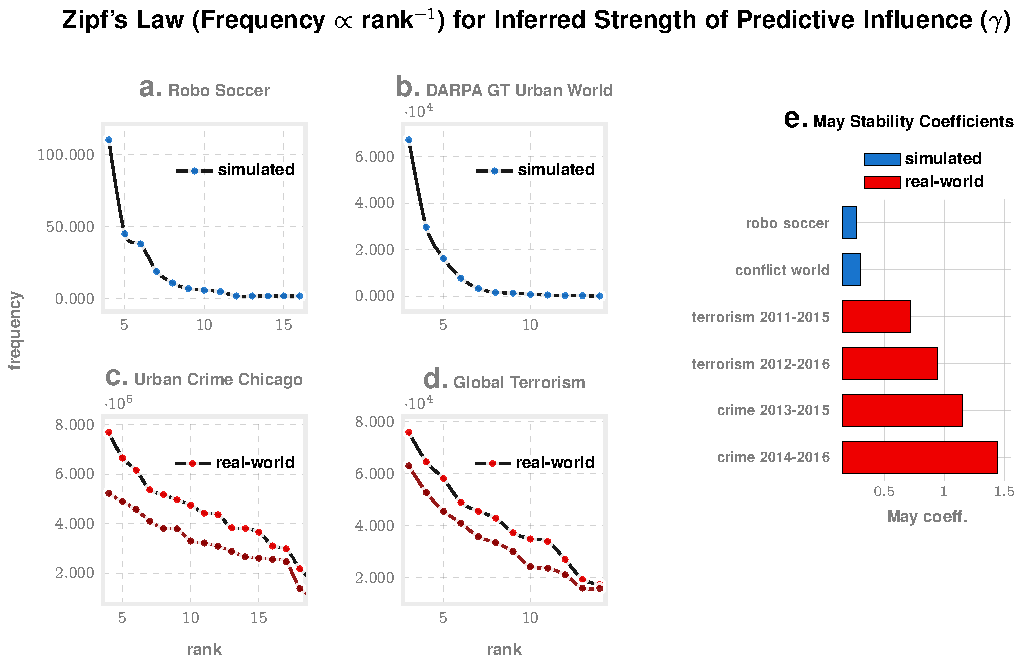
\includegraphics[width=1.02\textwidth]{Figures/External/main-figure0}
  \vspace{-25pt}

  \fi

  
  \captionN{Three Estimators from the Recursive Forest computed with a small number of query items from the GSS 2018. The items, as shown, ask if the person is strongly religious, if they support marijuana legalization, and if faculty with communistic ideologies should be fired from their teaching positions. Our calculations indicated a high dissonance for the questions on religion (A) and communism (B), and a low dissonance on cannabis legalization (C).  We note that further inspection, we find that both trees in A and B have clear dissonant patterns (marked in Red), while the tree for cannabis usage legalization does not. In particular, the decision tree in A indicates that there are individuals who pray multiple times a day, but consider themselves not very strongly religious. And B indicates that there are people who think faculty with communistic ideology should be fired, any text written by them should be removed from libraries (var: libcom), but also think that faculty supporting the military takeover of US and doing away with elections should be allowed to teach (var: colmil). Irrespective of whether these individual ideas can be supported, these results demonstrate our ability to uncover these potential dissonant patterns. In panel C, we have indications of both people supporting and disagreeing with cannabis legalization, but the views seem to be relatively free from obvious conflict. Inset shows that how the dissonance over the cannabis question has evolved over time, finally dropping below the mean dissonance level in 2016.}\label{fig0}
  \vspace{-20pt}
\end{figure}
% ###########################
% ###########################
\subsection*{Recursive Decision Forests From Survey Responses}
The recursive decision forest is a set of decision trees: given a survey with $N$ questions, the recursive forest consists of at most $N$ decision trees, where the $i^{th}$ tree attempts to predict the answers to the $i^{th}$ question using the responses to the rest of the $(N-1)$ questions as features.

Thus, in contrast to  random forests, the estimators in a recursive forest are not independent. Also,  recursive forests are not necessarily ensemble estimators per se, $i.e.$, unlike random forests, we are not attempting to improve prediction by averaging over a predictor ensemble;  we are trying to infer dependencies across features, $i.e.$, the observable characteristics of the system at hand.

The ``recursive'' nature of the forest arises from the fact that while the responses to  question $i$ might be affected by the responses to question $j$, the decision tree predicting $j$ might in turn use the responses to  $i$ as a predictive feature. Thus, the complete set of decision trees capture the potentially complex emergent dependencies between the survey responses. These dependencies may be inferred reliably even in the lack of any deep understanding of the nature of the questions, and the explicit societal forces that shape these structures. To describe the picture  formally, we need the following definitions:
% 
\def\I{\mathds{I}}
\def\D{\mathfrak{D}}
\def\Q{\mathds{Q}}
\def\R{X}
\def\supp{\mathop{\mathsf{supp}}}
\def\u{\boldsymbol{u}}
\begin{defn}[Item Set]
  Let $\I$ be a finite set of questions (items) presented to a population of individuals in the course of a survey. We call this the \textit{item set}.  Each item response can be either categorical, ordinal or real valued. The
  range of each item $i \in \I$ is denoted as $\Sigma_i$. 
\end{defn}
% 
We can think of $\I$ as the index set of a set of random variables, $i.e.$, the item $i \in \I$ indexes a random variable $X_i$ taking values in $\Sigma_i$. And, the response of a specific individual to a particular item $i \in \I$ is  a sample for the corresponding random  variable $X_i$. These random variables are not independent, and the task of the recursive forest is to infer these dependencies.
%% ###########################
% ###########################
% ###########################
\begin{figure}[!t]
  % \centering
  \vspace{-10pt}
  
  \iftikzX
  \hspace{-25pt}
  \input{Figures/clsmap.tex}
  \vspace{-22pt}
  \else \includegraphics[width=0.97\textwidth]{Figures/External/main-figure1}
  \vspace{-15pt}
  \fi

  
  \captionN{Dissonance measure used to find clusters with a limited set of survey questions from the years 2016  in the GSS dataset. We see that dissonance levels are mostly stable across people for most questions, but subtle changes make beliefs shift over time, as evidenced by the question on cannabis legalization in Fig.~\ref{fig0}}\label{fig1}
  \vspace{-20pt}
  
\end{figure}
% ###########################
% ###########################
% ###########################
% ###########################%
\subsubsection*{Recursive Forest Construction}
Let $\D\left (i,\I\setminus\{i\}\right )$ be a decision tree with  item $i$ as the target variable, and the rest of the  items acting as ``features'' on which  decision rules are imposed. Thus:
\cgather{
  \D\left (i,\I\setminus\{i\}\right ) = R_1\vee \cdots R_\ell \vee \cdots R_k
  \intertext{where $R_\ell$ are distinct rules, $i.e.$, paths from the root to a leaf in the decision tree:}
  \forall \ell, R_\ell = C_1 \wedge \cdots C_s \cdots \wedge C_m
  \textrm{ and }
  \forall s, \exists  j \in \I\setminus\{i\} , \textrm { s.t. } C_s \subset \Sigma_j
}
% The recursive forest is defined to be the collection of all such decision trees computed on $\I$.
% 
{\noindent}We  always use conditional inference trees~\cite{Sard-Espinosa:2017:CIT:3108944.3109065}, unless otherwise specified.  In contrast to decision tree construction algorithms that perform univariate splits and use information measures such as the gini coefficient to select covariates, conditional inference trees uses multiple significance test procedure based on permutations.
% 
\begin{defn}[Formal Definition of Recursive Decision Forest $\Q$] Using the notation introduced above, we define a recursive forest as the complete set of all cross-dependent predictors  computed on $\I$:
  \cgather{
    \Q \triangleq \bigg  \{  \D\left (i,\I\setminus\{i\}\right ), i \in \I \bigg \}
  }
\end{defn}
%%%%% 
\begin{notn}
  The set of features involved in the decision tree $\D$ is denoted as $\supp(\D)$.
  % Thus, $\supp(\D\left (i,\I\setminus\{i\}\right )) \subseteqq \I\setminus\{i\}$.
  Additionally, negative subscripts $e.g.$ $x_{-i}$ denote a vector $x_1,\cdots,x_{i-1},x_{i+1}, \cdots x_\I$, $i.e.$, excludes the index $i$.
\end{notn}
%%%% 
\begin{defn}[Conditional Cross-estimate]
  A conditional cross-estimate $\mu_i(\Q,X_{-i})$ for the $i^{th}$ item is a random variable conditioned on the inferred recursive forest $\Q$, and the recorded responses $X_{-i}=x_{-i}$ to the rest of the items in $\I$. Thus, in the categorical case, we have:
  \cgather{
    Pr(\mu_i(\Q,X_{-i}) = \sigma \in \Sigma_i) = Pr(X_i = \sigma \vert X_{-i}=x_{-i}, \Q)
  }
  The definition  for  ordinal and continuous variables is analogous.
\end{defn} 
% 
\subsection*{Quantitative Definition of Cognitive Dissonance As A Large Deviation Estimate}
We use large deviation theory to estimate the surprise in a recorded response from the
its conditional cross-estimate, to quantify dissonance. Thus:
\begin{defn}[Dissonnance Vector $\u$]
  For a specific individual, the dissonance measure $\u_i$ at item $i\in \I$, given  the inferred recursive forest $\Q$, and the responses $x_i, i \in \I$ is given by:
  \cgather{
    \u_i(x_i,x_{-i},\Q) = 1 - 2^{Pr(\mu_i(\Q,X_{-i})=x_i)\log_2 Pr(\mu_i(\Q,X_{-i})=x_i)}    
  }
  where the second term on the right hand side is the probability  of the observed deviation of the conditional cross-estimate and the actual response $x_i$ from large deviation theory and Sanov's theorem~\cite{cover}. Note that, as per notation, $x_i$ is the response to the $i^{th}$ item, whereas $x_{-i}$ is the vector of responses to the rest of the items indexed by $\I$.
\end{defn}
The  dissonance vector generalizes readily to scenarios where we are interested in   a community or a sub-population instead of individual respondents, and where only a subset of responses are available.

The ability to  infer dissonance is demonstrated in Fig.~\ref{fig0}, with $3$ trees inferred from GSS 2018 survey data. Our analysis suggested that the trees in panels A and B had a high dissonance value, while the one is panel C (support of cannabis legalization) did not. Inspecting the trees, we find immediate evidence of conflict as shown highlighted in red (See figure caption for details). Fig.~\ref{fig1} illustrates the variation in dissonance across people, and survey questions.
% 
\subsection*{Predicting Dissonance Response: Trivialization or Change in Belief?}
Festinger's thesis dictates that dissonance motivates actions for reducing conflict. With the formal definition of  the dissonance vector, we can work out the probabilities of the different categories of  response strategies invoked by an individual. %We estimate the probabilities that the response to dissonance will be either a change in beleifs, or something else akin to trivialization or attempted rationalization of current beliefs.
In particular, we investigate the probability of  dissonance dissipation by perturbing the specific responses. If a perturbation in the recorded response alone for the $i^{th}$ item is able to effectively reduce the value of the dissonance vector at $i$, then changing one's beliefs is a viable strategy. Likewise, if  a perturbation in  the responses to the rest of the items  reduces dissonance, then  some form of rationalization or trivialization is also viable.
To estimate the likelihood of trivialization, we assume that individuals tend to follow the path of least resistance.  Thus, we ask, that given the current dissonance $ \u_i^\star$ in the item $i \in \I$:
\begin{itemize}
\item How hard is it to reduce dissonance holding  $X_i$ constant, $i.e.$, estimate $\alpha_{i,\Q} \triangleq Pr(\u_i \leqq \u_i^\star \vert X_i)$
\item How hard is it to reduce dissonance holding $X_{-i}$ constant, $i.e.$, estimate $\beta_{i,\Q} \triangleq Pr(\u_i \leqq \u_i^\star \vert X_{-i})$
\end{itemize}
The  probability of  adopting trivialization/rationalization is then the marginalized estimate:
\cgather{
  \wp_{i,\Q} \triangleq \frac{\alpha_{i,\Q} }{\alpha_{i,\Q} +\beta_{i,\Q}}
}
Clearly, it is harder to change one's beliefs as opposed to rationalization: perturbing a single response to achieve reduction in $\u_i$ is  harder to achieving the same by perturbing thousands of variables instead.
\subsection*{Master Equation for Long Term Evolution Dynamics of Belief Shift}
To model the dynamics of belief shift over time, we will investigate a range of increasingly complex  approaches that progressively relax simplifying assumptions.
The analysis outlined above, in conjunction with Festinger's notion that belief shifts due to cognitive dissonance are aimed as reducing the current conflict, leads to the following stochastic evolution equations:
\calign{
  &  Pr(X_i^{t+\Delta t} = X_i^t) = \wp_{i,\Q_t} \label{eq7} \\
  &  Pr(X_i^{t+\Delta t} = x) = \left \{ \begin{array}{ll} c_t (\u_{i}(x,x_{-i},\Q_t) - \u_{i}(x_i,x_{-i},\Q_t)), & \textrm{if } \u_{i}(x,x_{-i},\Q_t) < \u_{i}(x_i,x_{-i},\Q_t) \\
                                           0, & \textrm{otherwise} \end{array} \right. \label{eq8} \\
                                       & \textrm{where } c_t= (1 - \wp_{i,\Q_t}) \left (  \sum_{x \in \Sigma_i}  \left (   \u_{i}(x,x_{-i},\Q_t) - \u_{i}(x_i,x_{-i},\Q_t)  \right ) \right )^{-1} \notag
                                     }
                                     \noindent These relationships may be cast as a generalized Master Equation, often used to model stochastic dynamics. Note, Eq.~\eqref{eq7} is the \textbf{rationalization dynamics} (probability of no change in beliefs), and Eq.~\eqref{eq8} \textbf{models the shift in beliefs}, using Festinger's diktat that the dissonance measure must decrease. In our initial investigations, we assume that the probability of shifting to a new belief is proportional to the decrease in dissonance. Since no shift in belief for $X_i$ $i.e.$ the rationalization or trivialization action might change responses in other items (in the set $X_{-i}$), the dynamics is  coupled across items, leading to  complex stochastic evolution. One of our core objectives will be to investigate efficient solutions of this set of equations, and validate  results directly in longitudinal survey data.    Additionally, we will consider  frameworks with hidden states to model more complex responses.                           
                                     \subsection*{Research Plan}
                                     Our research plan consists of  development of inference algorithms as outlined above, with  consequent validation in large scale social survey data sets. The two main data sets to be used in this context are 1) the General Social Survey (GSS) , and 2) the National Longitudinal Study of Youth (NLSY).
                                     % 
                                     \subsubsection*{GSS Dataset} The National Data Program for the Social Sciences has been conducted since 1972 by the non-partisan and objective research organization (NORC,\href{http://www.norc.org}{http://www.norc.org}) at the University of Chicago,  with the support of the National Science Foundation. %The GSS gathers data on contemporary American society in order to monitor and explain trends and constants in attitudes, behaviors, and attributes.
                                     The GSS contains a standard core of demographic, behavioral, and attitudinal questions, plus topics of special interest, and will be used as the main development, tuning and validation data for our learning algorithms. While individual belief shifts cannot be directly validated, population level predictions of the belief evolution over time will be tested on the GSS data.
                                     % 
                                     \subsubsection*{NLSY Data set} The NLSY79 Cohort (\href{https://www.nlsinfo.org/content/cohorts/nlsy79}{https://www.nlsinfo.org/content/cohorts/nlsy79}) is a longitudinal project maintained by the U.S. Bureau of Labor Statistics, that follows the lives of a sample of American youth born between 1957-64. The cohort originally included 12,686 respondents ages 14-22 when first interviewed in 1979; after two sub-samples were dropped, 9,964 respondents remain in the eligible samples. %Data are now available from Round 1 (1979 survey year) to Round 27 (2016 survey year).
                                     The NLSY data set is of crucial importance to our proposed validation goals of predicting belief shifts over time, in response to quantified dissonance measures.

                                     The planned research comprises the following tasks:
                                     \begin{enumerate}
                                       [label=\tball, leftmargin=0pt,
                                       labelindent=0em, topsep=0.1em, labelsep=*, itemsep=.75em,itemindent=2em]\color{CadetBlue4!40!black} \sffamily\fontsize{11}{12}\selectfont
                                     \item  \textbf{Task 1 (Recursive Forest Generation)} The recursive forest generation task involves developing the general theory of recursive decision forests, and adopting the framework to sociological survey data. Key challenges here as scalability, identifying theoretical bounds on uncertainties, and sample complexities, and understanding trade-offs between the complexity of individual decision trees, and the predictive performance. We will also explore replacing decision trees as the component estimators in the recursive forest with more advanced predictors, $e.g.$, random forests (resulting in a recursive forest of random forests), gradient boosting ensembles, and multi-layer feed-forward perceptron networks.
                                     \item  \textbf{Task 2 (Belief Shift Prediction \& Validation)} The belief propagation task will investigate the dynamics of belief evolution over time, as predicted by the inferred decision forests, and the computational approaches outlined in the previous section. 
                                     \item  \textbf{Task 3 (Software Development \& Validation)} This task focuses on developing efficient software implementations, that ultimately can be used easily by researchers and other  DoD programs.
                                     \item  \textbf{Task 4 (Experimental Validation)}
                                       Finally, we will carry out focused experiments with human subjects recruited from university of Chicago campus, and its surrounding locale in the City of Chicago, to carry out belief shift experiments in a controlled environment. Appropriate IRB approvals will be sought before the experiments are conducted.
                                     \end{enumerate}
                                     \subsection*{Measurable Milestones for Tracking Progress}
                                     % Research progress may be tracked via the following  measurable milestones:
                                     \begin{enumerate}
                                       [label=\tball, leftmargin=0pt,
                                       labelindent=0em, topsep=0.1em, labelsep=*, itemsep=.15em,itemindent=2em]\color{black} \sffamily\fontsize{11}{12}\selectfont
                                     \item  \textbf{Milestone 1 (month 3)} Initial software development complete, ready for analysis of survey data.
                                     \item  \textbf{Milestone 2 (month 6)} Recursive forests computed for GSS years from 1972 to 2018.
                                     \item \textbf{Milestone 3 (month 6) } Demonstration of belief shift dynamics in synthetic scenarios.
                                     \item  \textbf{Milestone 4 (month 12)} Dissonance measures and rationalization probability calc. demonstrated.
                                     \item \textbf{Milestone 5 (month 18) } Analysis of longitudinal data sets complete
                                     \item \textbf{Milestone 6 (month 24} Demonstration of validated belief shift dynamics in longitudinal data sets.
                                     \item \textbf{Milestone 7 (month 24)} Software deliverable at 2 year mark
                                     \item \textbf{Milestone 8 (month 30)} Belief shift calculations  with relaxed assumptions demonstrated.
                                     \item \textbf{Milestone 9 (month 30)} Initial reports from focused experiments reported.
                                     \item \textbf{Milestone 10 (month 36)} Validated software implementation reported for overall project.
                                     \item \textbf{Milestone 11 (month 36)} Analysis of experimental results reported, Final report submitted.
                                     \end{enumerate}
                                     % 
                                     \subsection*{Technical Risk \& Mitigation}
                                     Our key technical risk are potential flaws in the theory of cognitive dissonance. We will mitigate this risk by suitably modifying our belief shift equations, and possibly even back out the driving equations from longitudinal data sets via machine learning approaches, at the cost of increased uncertainties.
                                     \section{Management Plan}
                                     \begin{enumerate}
                                       [label=\tball, leftmargin=0pt,
                                       labelindent=0em, topsep=0.1em, labelsep=*, itemsep=.25em,itemindent=2em]\color{black} \sffamily\fontsize{11}{12}\selectfont
                                     \item \textbf{Prof. Ishanu Chattopadhyay, PhD (Principal Investigator, Effort: 30-40\%):} is an expert in machine learning, stochastic processes, and predictions and forecasting in complex biological and social systems. Dr. Chattopadhyay, with help from two post-doctoral associates,  will be responsible for all theoretical development, software implementation, and data management. 
                                     \item \textbf{Prof. James Allen, PhD (Subject Matter \& Data Expert, Effort: 5\%):} is a professor of  sociology at the University of Chicago, and is an expert in social theory, computational sociology, and big data analysis. Professor Evans will advise on social theory, interpretation of variable associations inferred by the proposed algorithms in survey data,  and help the PI in designing the human subject experiments.
                                     \item \textbf{Post doctoral Researcher 1 (Effort 100\%):} will report to the PI, and be responsible for theoretical development  of recursive forests, and uncertainty quantification in belief evolution.
                                     \item \textbf{Post doctoral Researcher 2 (Effort 85\%):} will report to the PI, and be responsible for software development, and validation and tuning of the framework on large scale data sets.
                                     \end{enumerate}
                                     % Provide a summary of expertise of the key personnel on the proposed team (including any subcontractors and consultants) who will be executing the work.  Identify a principal investigator (PI) for the project.  
                                     % Provide a clear description of the team’s organization including an organization chart that includes, as applicable, the relationship of team members; unique capabilities of team members; task responsibilities of team members; teaming strategy among the team members; and key personnel with the amount of effort to be expended by each person during the project.  
                                     % Provide a detailed plan for coordination including explicit guidelines for interaction among collaborators/subcontractors of the proposed project.  Include risk management approaches.  
                                     % Describe any formal teaming agreements that are required to execute this project.
                                     \section{Personnel, Qualifications, and Commitments}
                                     \textbf{Prof. Chattopadhyay (PI): (Level of Effort: 560 hr/yr in base, 768 hr/yr in option) } 
                                     Dr. Chattopadhyay has a diverse background in machine learning, stochastic processes and systems biology, and has multiple graduate degrees in engineering, computer science, and mathematics. He earned his doctoral degree from the Pennsylvania State University, and completed his postdoctoral training at Cornell University. As a faculty in University of Chicago, Chattopadhyay heads the laboratory for Zero Knowledge Discovery (zed.uchicago.edu), where his research focuses on learning theory, and the modeling of complex systems.  His most visible contributions include the algorithms for data smashing~\cite{Chattopadhyay20140826}, inverse Gillespie inference~\cite{Chattopadhyay12990},  non-parametric implementations of Granger  inference~\cite{DBLP:journals/corr/Chattopadhyay14}, and the modeling and prediction of complex social phenomena including urban crime~\cite{li2019longrange} Chattopadhyay is currently funded by DARPA (total 30\% effort), and has been previously supported by  the Neubauer Collegium for Culture and Society {\footnotesize (\href{https://neubauercollegium.uchicago.edu/events/uc/crimes\_of\_prediction/}{https://neubauercollegium.uchicago.edu/events/uc/crimes\_of\_prediction}}).
                                     Curriculum Vitae is linked in the Bibliography.

                                     \textbf{Prof. Evans} has multiple funded grants including with DARPA. His CV is linked in the Bibliography.
                                     % List key personnel (no more than one page per person), showing a concise summary of their qualifications, discussion of previous accomplishments, and work in this or closely related research areas.  Do not include personnel that are not anticipated to execute the work.
                                     % Indicate the level of effort in terms of hours to be expended by each person during each year and other (current and proposed) major sources of support for them and/or commitments of their efforts.
                                     \section{Capabilities}
                                     University of Chicago has extensive computational facilities. The NORC at the University of Chicago is an objective non-partisan research institution that maintains the GSS database. Likewise, the National Longitudinal Survey of Youth (NLSY), is  conducted jointly by the Ohio State University and the NORC.
                                     % Describe organizational experience in relevant subject area(s), existing intellectual property, or specialized facilities.  Discuss any work in closely related research areas and previous accomplishments.  
                                     % 
                                     % Identify any other solicitation(s) to which this concept has been proposed.  If applicable, state whether funding or a positive funding decision has already been received, and from which agency.

                                     % \clearpage
                                     \cfoot{}
                                     \section{Statement of Work (SOW)}
                                     All work will be performed at the University of Chicago, under the supervision of Dr. Chattopadhyay.
                                     \subsubsection*{Task 1 Year 1}
                                     \textbf{Objective:} Recursive Decision Forest Models\\
                                     \textbf{Description:} Development of the theory of recursive decision forests, and demonstrate applicability to GSS dataset. Demonstrate dissonance calculation, and estimation of probability of rationalization vs opinion change on GSS dataset.
                                     \textbf{Milestones:} 2 (Month 6), 4 (Month 12)
                                     \vspace{-5pt}

                                     \subsubsection*{Task 2 Year 1}\textbf{Objective:} Belief Shift Prediction in Simple Scenarios\\
                                     \textbf{Description:} Demonstration of belief shift dynamics in synthetic scenarios 
                                     \textbf{Milestones:} 3 (Month 6)
                                     \vspace{-5pt}

                                     \subsubsection*{Task 3 Year 1} \textbf{Objective:} Software Implementation\\
                                     \textbf{Description:} Beta Implementation of Recursive Decision Forests without efficiency and
                                     robustness considerations.\textbf{ Milestones:} 1 (Month 3)
                                     \vspace{-5pt}

                                     \subsubsection*{Task 1 Year 2}
                                     \textbf{Objective:} Recursive Decision Forest Models for Longitudinal Data sets\\
                                     \textbf{Description:} Development of strategies to analyze time varying recursive forests to analyze longitudinal data sets including the NLSY dataset.
                                     \textbf{Milestones:} 5 (Month 18)
                                     \vspace{-5pt}

                                     \subsubsection*{Task 2 Year 2}\textbf{Objective:} Belief Shift Prediction with relaxed assumptions\\
                                     \textbf{Description:} Demonstration of belief shift dynamics in the GSS and the NLSY \\
                                     \textbf{Milestones:}  6 (Month 24)
                                     \vspace{-5pt}

                                     \subsubsection*{Task 3 Year 2} \textbf{Objective:} Software Implementation with validation\\
                                     \textbf{Description:} Version 1.0 Implementation of Recursive Decision Forests with efficiency and robustness considerations.\textbf{ Milestones:} 7 (Month 24)
                                     \vspace{-5pt}

                                     \subsubsection*{Task 1 Year 3}
                                     \textbf{Objective:} Advanced Recursive Decision Forest Models for Longitudinal Data sets\\
                                     \textbf{Description:} Develop theoretical bounds on sample complexities, convergence rates, and investigate changing the base estimators to random forests, boosting classifier, and multi-layer perceptrons.
                                     \textbf{Milestones:} 10 (month 36), Report submitted
                                     \vspace{-5pt}

                                     \subsubsection*{Task 2 Year 3}\textbf{Objective:} Advanced Belief Shift Prediction\\
                                     \textbf{Description:} Demonstration of belief  dynamics in  GSS and  NLSY.
                                     \textbf{Milestones:}  8 (Month 30)
                                     \vspace{-5pt}

                                     \subsubsection*{Task 3 Year 3} \textbf{Objective:} Software Implementation with validation\\
                                     \textbf{Description:} Version 2.0 Implementation of Recursive Decision Forests with  the ability to optimize the base estimator class.\textbf{ Milestones:}  10 (Month 36)
                                     \vspace{-5pt}

                                     \subsubsection*{Task 4 Year 3} \textbf{Objective:} Human Subject Experiments\\ \textbf{Description:} Selecting random subjects from university campus and surrounding areas, and carry out longitudinal survey with carefully crafted questions. \\  IRB approval will be sought. \textbf{Milestones:} 9 (month 30), 11 (month 36)

                                     % provide a detailed task breakdown, citing specific tasks and their connection to the proposed milestones.  The SOW task structure must be consistent with the schedule, milestones and costs.  Separately define each year of the project.  Do not include any proprietary information. For each defined task/subtask/activity, provide:
                                     % A general description of the objective.
                                     % A detailed description of the approach to be taken to accomplish each defined task/subtask (including, where applicable, identifying the tasks/subtasks that will be performed on campus at a university).
                                     % Identification (by name) of the primary organization (prime contractor, subcontractor(s), consultant(s)) responsible for task/subtask execution.
                                     % A measurable milestone, (e.g., a deliverable, demonstration, or other event/activity that marks task completion).
                                     % A definition of all deliverables (e.g., data, reports, software) to be provided to the Government in support of the proposed tasks/subtasks.

                                     \section{Schedule and Milestones}
                                     % Provide a detailed schedule showing tasks (task name, duration, work breakdown structure element as applicable, performing organization), milestones, and the interrelationships among tasks.  The task structure must be consistent with that in the SOW.  Measurable milestones should be clearly articulated and defined in time relative to the start of the project.

                                     \begin{center}

                                       Milestones shown in red.
                                       
                                       \tikzexternaldisable
                                       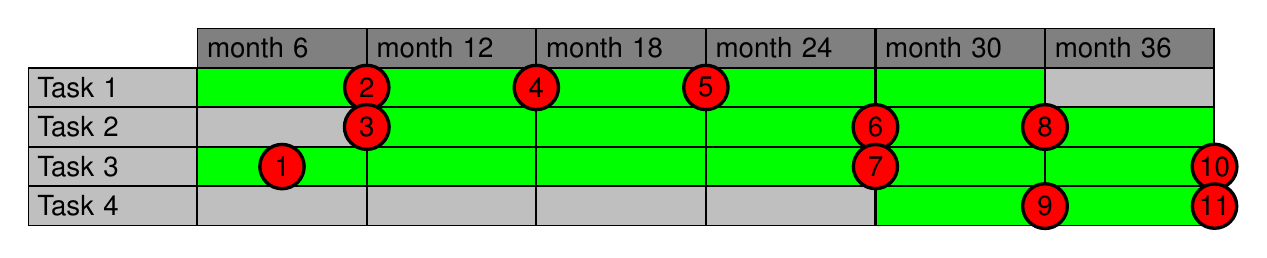
\begin{tikzpicture}
                                         \def\CGOL{lightgray}
                                         \def\FCOL{Green1}
                                         \tikzstyle{ann} = [draw=,fill=\CGOL,text width=.75in, text height=.1in,anchor=north]
                                         \tikzstyle{mls} = [circle,anchor=center, fill=Red1, draw=black, text width=.2in, align=center,inner sep=0pt, very thick]
                                         \node[ann,fill=gray] (Y10) at (0,0) {month 6};
                                         \node[ann,fill=\FCOL] (T1Y10) at (Y10.south) {};
                                         \node[ann] (T2Y10) at (T1Y10.south) {};
                                         \node[ann,fill=\FCOL] (T3Y10) at (T2Y10.south) {};
                                         \node[ann] (T4Y10) at (T3Y10.south) {};

                                         \node[mls] (M1) at (T3Y10.center) {1};


                                         
                                         \node[ann,fill=gray,anchor=west] (Y11) at (Y10.east) {month 12};
                                         \node[ann,fill=\FCOL] (T1Y11) at (Y11.south) {};
                                         \node[ann,fill=\FCOL] (T2Y11) at (T1Y11.south) {};
                                         \node[ann,fill=\FCOL] (T3Y11) at (T2Y11.south) {};
                                         \node[ann] (T4Y11) at (T3Y11.south) {};


                                         \node[ann,fill=gray,anchor=west] (Y20) at (Y11.east) {month 18};
                                         \node[ann,fill=\FCOL] (T1Y20) at (Y20.south) {};
                                         \node[ann,fill=\FCOL] (T2Y20) at (T1Y20.south) {};
                                         \node[ann,fill=\FCOL] (T3Y20) at (T2Y20.south) {};
                                         \node[ann] (T4Y20) at (T3Y20.south) {};

                                         
                                         \node[ann,fill=gray,anchor=west] (Y21) at (Y20.east) {month 24};
                                         \node[ann,fill=\FCOL] (T1Y21) at (Y21.south) {};
                                         \node[ann,fill=\FCOL] (T2Y21) at (T1Y21.south) {};
                                         \node[ann,fill=\FCOL] (T3Y21) at (T2Y21.south) {};
                                         \node[ann] (T4Y21) at (T3Y21.south) {};

                                         \node[ann,fill=gray,anchor=west] (Y30) at (Y21.east) {month 30};
                                         \node[ann,fill=\FCOL] (T1Y30) at (Y30.south) {};
                                         \node[ann,fill=\FCOL] (T2Y30) at (T1Y30.south) {};
                                         \node[ann,fill=\FCOL] (T3Y30) at (T2Y30.south) {};
                                         \node[ann,fill=\FCOL] (T4Y30) at (T3Y30.south) {};

                                         
                                         \node[ann,fill=gray,anchor=west] (Y31) at (Y30.east) {month 36};
                                         \node[ann] (T1Y31) at (Y31.south) {};
                                         \node[ann,fill=\FCOL] (T2Y31) at (T1Y31.south) {};
                                         \node[ann,fill=\FCOL] (T3Y31) at (T2Y31.south) {};
                                         \node[ann,fill=\FCOL] (T4Y31) at (T3Y31.south) {};


                                         % \node[ann,fill=gray] (Y10) at (0,0) {month 6};
                                         \node[ann,anchor=east] (T1) at (T1Y10.west) {Task 1};
                                         \node[ann,anchor=east] (T2) at (T2Y10.west) {Task 2};
                                         \node[ann,anchor=east] (T3) at (T3Y10.west) {Task 3};
                                         \node[ann,anchor=east] (T4) at (T4Y10.west) {Task 4};

                                         \node[mls] (M2) at (T1Y10.east) {2};
                                         \node[mls] (M3) at (T2Y10.east) {3};
                                         \node[mls] (M4) at (T1Y11.east) {4};
                                         \node[mls] (M5) at (T1Y20.east) {5};
                                         \node[mls] (M6) at (T2Y21.east) {6};
                                         \node[mls] (M7) at (T3Y21.east) {7};
                                         \node[mls] (M8) at (T2Y30.east) {8};
                                         \node[mls] (M9) at (T4Y30.east) {9};
                                         \node[mls] (M10) at (T3Y31.east) {10};
                                         \node[mls] (M11) at (T4Y31.east) {11};

                                       \end{tikzpicture}

                                     \end{center}
                                     % \clearpage


                                     % \input{Figures/treemap2.tex}


                                     \clearpage 
                                     % \setcounter{page}{1}
                                     \section{Bibliography}
                                     % Optional.  If desired, include links to relevant papers, reports or resumes.  Do not include technical papers. The linked materials will not be evaluated as part of the proposal review

                                     CV for Ishanu Chattopadhyay:

                                     \href{https://zed.uchicago.edu/cv/chattopadhyay\_cv.pdf}{https://zed.uchicago.edu/cv/chattopadhyay\_cv.pdf}

                                     CV for Other Personnel:

                                     \href{https://www.knowledgelab.org/}{https://www.knowledgelab.org/}

                                     \bibliographystyle{naturemag}
                                     \bibliography{creed,qnet,BibLib1}

                                   \end{document}
                                   % ####################################
                                   % ####################################
                                   % ####################################
                                   % ####################################
                                   % ####################################
                                   % ####################################
                                   % ####################################
